\textbf{COLUNI 2021 -- Questão 38}\par\medskip O processo de colonização da África e da Ásia foi conduzido por países europeus em função de interesses econômicos e políticos, especialmente com objetivo de conquistar novos mercados consumidores, acesso a matérias primas e domínio colonial. Tal processo foi nomeado de colonialismo. Por outro lado, os povos africanos e asiáticos resistiram à colonização, movimento que se acelerou com o término da Segunda Guerra Mundial e levou à independência das regiões dominadas.

\par

Sobre os movimentos de resistência e de independência no continente africano, observe as imagens abaixo:

\par

\begin{minipage}[t]{0.48\linewidth}\centering
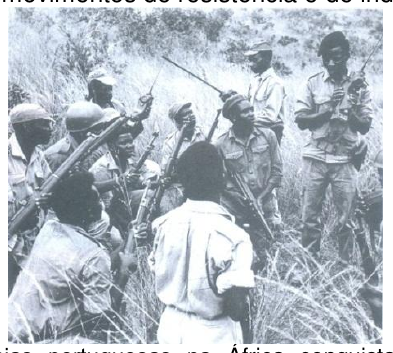
\includegraphics[width=\linewidth]{static/simulados/coluni/figuras/2021/questao-38/figura-1.png}\par
“As colônias portuguesas na África conquistaram sua independência apenas a partir de 1974, após anos de luta contra o exército português. Nessa fotografia, vemos guerrilheiros anticoloniais de Angola em 1964.”\par
PELLEGRINI, Marco; DIAS, Adriana; GRINBERG, Keila. \textbf{Vontade de saber história}, 9º ano. 2. ed. São Paulo: FTD, 2012, p. 161.
\end{minipage}\hfill
\begin{minipage}[t]{0.48\linewidth}\centering
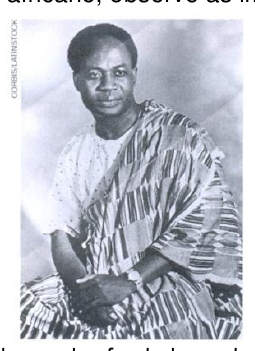
\includegraphics[width=\linewidth]{static/simulados/coluni/figuras/2021/questao-38/figura-2.png}\par
“Kwame Nkrumah, um dos fundadores do pan-africanismo e líder do movimento de independência de Gana. Na ocasião desse retrato, feito em 1959, ele ocupava o cargo de primeiro-ministro de Gana.”\par
BRAICK, Patrícia Ramos. \textbf{Estudar História 9}: das origens do homem à era digital. 2ª. ed. São Paulo: Moderna, 2015, p. 172.
\end{minipage}

\medskip

\begin{minipage}[t]{0.48\linewidth}\centering
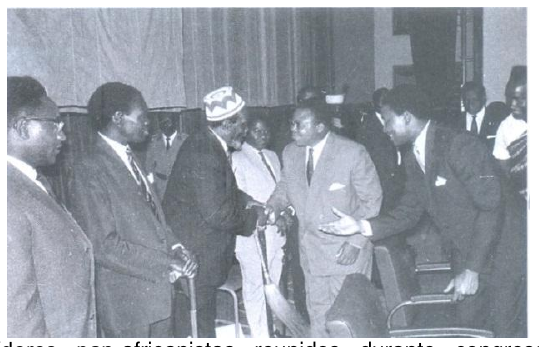
\includegraphics[width=\linewidth]{static/simulados/coluni/figuras/2021/questao-38/figura-3.png}\par
“Líderes pan-africanistas reunidos durante congresso realizado no Congo, em 1962.”\par
PELLEGRINI, Marco; DIAS, Adriana; GRINBERG, Keila. \textbf{Vontade de saber história}, 9º ano. 2. ed. São Paulo: FTD, 2012, p. 161.
\end{minipage}\hfill
\begin{minipage}[t]{0.48\linewidth}\centering

\includegraphics[width=\linewidth]{static/simulados/coluni/figuras/2021/questao-38/figura-4.png}\par
“Sul-africana deixa banheiro reservado para mulheres não brancas durante o regime do apartheid. Soweto, África do Sul, 1970.”\par
BRAICK, Patrícia Ramos. \textbf{Estudar História 9}: das origens do homem à era digital. 2ª. ed. São Paulo: Moderna, 2015, p. 176.
\end{minipage}

\par

Sobre a resistência ao colonialismo e os movimentos de independência do continente africano, é INCORRETO afirmar que:


\begin{enumerate}
\item Os movimentos de afirmação da identidade africana desenvolveram-se desde o final do século XIX com a
      fundação da Associação Africana e a organização das Conferências Pan-Africanas, cujo objetivo era a
      luta contra o racismo e a garantia da soberania das colônias africanas e asiáticas.
\item A perda de prestígio e de capacidade militar e econômica dos países europeus envolvidos na Segunda
      Guerra Mundial provocou intenso abalo com relação aos domínios coloniais, resultando na ampliação das
      mobilizações em diferentes colônias da África e da Ásia em defesa da libertação nacional.
\item As ações políticas dos povos africanos, levadas a cabo pelas elites intelectuais nativas, como Kwame
      Nkrumah, tiveram pouco impacto nos movimentos de independência, a exemplo da independência de
      Gana, em 1957, primeiro país africano a se emancipar.
\item As leis segregacionistas impostas à população negra da África do Sul são resultado das decisões políticas
      dos africânders em 1920 e do regime de apartheid estabelecido em 1950 pelo Parlamento sul-africano,
      cujos resultados trouxeram graves consequências para a população desse país.\end{enumerate}
